\apendice{Documentación técnica de programación}

\section{Introducción}

\section{Estructura de directorios}

\section{Manual del programador}

\section{Compilación, instalación y ejecución del proyecto}

\section{Compilación, instalación y ejecución de herramientas auxiliares}

\subsection{KEEL}

\textit{KEEL} es una herramienta que permite experimentar con modelos de \textit{machine learning}. Ha sido creada por distintas universidades españolas y financiada por el Ministerio de Educación y Ciencia~\cite{KEEL}.

Para poder ejecutarla, en primer lugar, se han de descargar los ficheros fuente del repositorio de GitHub~\cite{keelRepo}. Una vez se han descargado, se compilan aprovechando el fichero \texttt{build.xmlz} contenido y la herramienta \texttt{ant}. Mediante el comando \texttt{ant cleanAll} se eliminan barios previos (para evitar conflictos), y mediante el comando \texttt{ant} se compila el código fuente.

Posteriormente se ejecuta la aplicación mediante el comando \texttt{java -jar ./dist/GraphInterKeel.jar} y se utiliza mediante su interfaz gráfica.

\begin{figure}[h]
	\caption{Configuración de un experimento que utiliza el algoritmo \textit{co-forest} mediante la \textit{GUI} de \textit{KEEL}.}
	\centering
	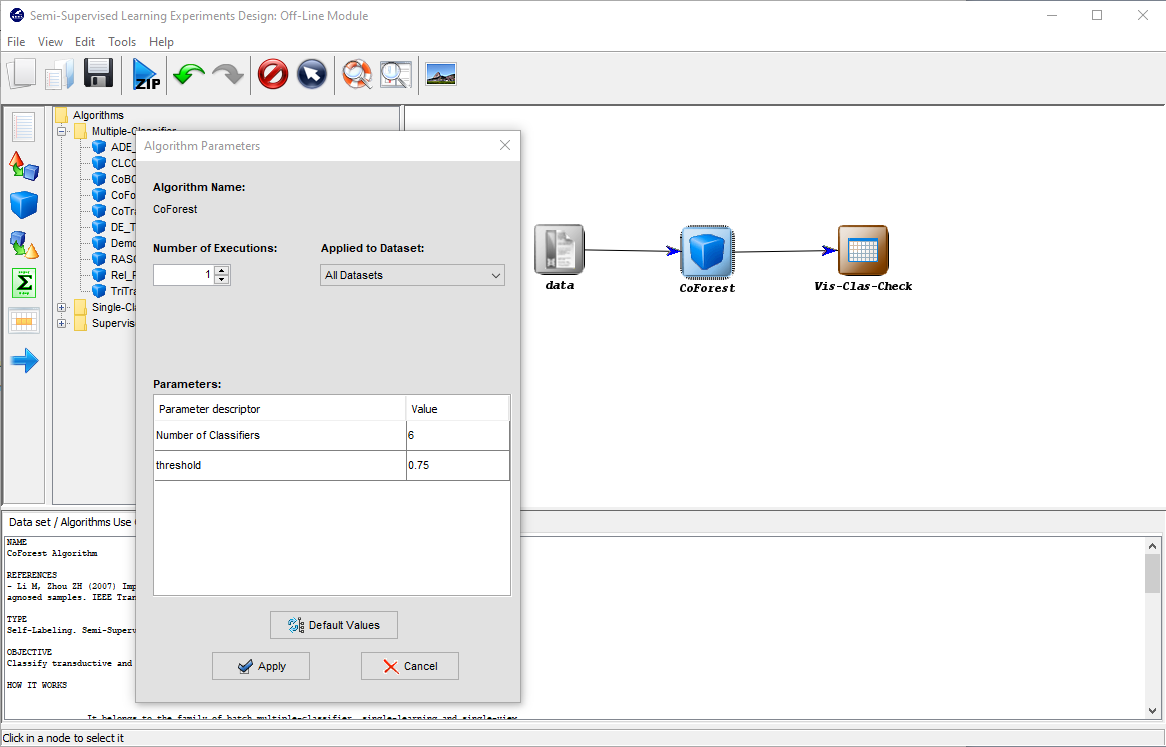
\includegraphics[width=\textwidth]{../img/anexos/manual/keel_gui.png}
\end{figure}


\section{Pruebas del sistema}
